\chapter{PROTOTYPE CSV VÀ KIỂM CHỨNG SUY LUẬN}\label{chap:demo}
\section{Mục tiêu và phạm vi sản phẩm}
Prototype giúp người xem đi từ một dòng dữ liệu mạng đến score, ngưỡng và dự đoán Normal/Attack. Người dùng chọn một trong bốn kịch bản CS/LR/LD/LE, một trong bốn mô hình RF/XGB/IF/AE và target FPR validation 1\% hoặc 5\%. Phần suy luận dùng bundle seed 42 đã lưu, không fit lại preprocessing, huấn luyện lại mô hình hoặc chọn ngưỡng từ CSV đang mở. Đầu vào mô hình gồm đúng 42 feature; metadata id, label và attack\_cat chỉ dùng truy vết, đối chiếu.

Đây là minh họa suy luận từ CSV có schema phù hợp UNSW-NB15. Sản phẩm chưa thu traffic trực tiếp, chưa tự học, chưa chặn tấn công và chưa có bộ dữ liệu mạng độc lập do nhóm tự thu thập. CSV mới theo nghĩa tệp vừa tải lên không tự trở thành dữ liệu độc lập; cần biết nguồn, cách trích feature và nhãn trước khi dùng để đánh giá.

\section{Giao diện trình bày trên laptop}
Giao diện tại \url{http://127.0.0.1:4397/presentation/} có bảy màn: Bài toán, Dữ liệu, Thực nghiệm, Kết quả, Demo, Hỏi đáp và Tự đánh giá. Người trình bày chuyển bằng nút tên mục hoặc phím mũi tên trái/phải. Hỏi đáp hiển thị một câu trả lời tại một thời điểm. Ghi chú lời nói mở riêng và đóng bằng Escape. Các nội dung này hỗ trợ trình bày phương pháp, bằng chứng và giới hạn, không thay cho phần giải thích của thành viên.

Màn Demo tách thành ba nút: ``Chọn dữ liệu'', ``Xem kết quả'' và ``Phạm vi demo''. Chạy thành công tự mở kết quả; quay lại bước chọn giữ cấu hình và tệp đã chọn. Khi thay cấu hình, kết quả cũ bị vô hiệu để tránh đọc nhầm. Nguồn của lần chạy và giới hạn nằm trong mục Phạm vi demo. Mục kết quả cho xem từng bản ghi, score so với ngưỡng, dự đoán, nhãn đối chiếu nếu có, số TP/FP/TN/FN và tải CSV.

Giao diện dùng nền sáng, một hệ chữ và điều hướng theo màn để hạn chế cuộn khi thuyết trình. Lần kiểm ngày 13/11 ghi nhận cả bảy màn vừa các khung 714\(\times\)667, 700\(\times\)600, 1366\(\times\)768 và 1920\(\times\)1080 pixel. Đây là kiểm trong trình duyệt, chưa phải xác nhận chất lượng máy chiếu hoặc kết nối HDMI thực tế. Ảnh~\ref{fig:presentation-current} ghi một lần suy luận thật trong giao diện mới.

\begin{figure}[H]\centering
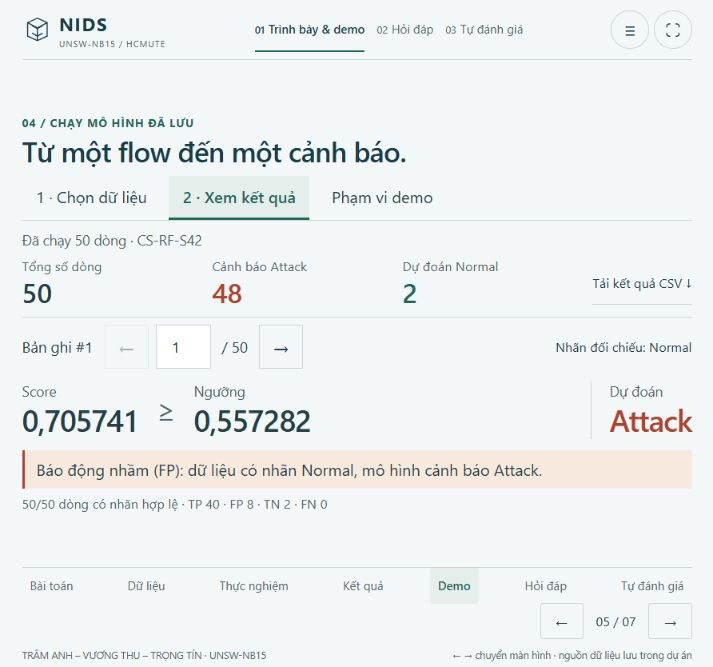
\includegraphics[width=\textwidth]{assets/presentation_20261113/DEMO_RESULT_714.jpg}
\caption[Màn Demo ngày 13/11, CS--RF seed 42, target validation 5\%]{Màn Demo ngày 13/11 trong khung Codex: CS--RF, seed 42, target validation 5\%, bộ hỗn hợp 50 dòng. Bản ghi 1 có nhãn Normal nhưng được cảnh báo Attack nên là FP. Số liệu trên mẫu minh họa không thay kết quả toàn test.}\label{fig:presentation-current}
\end{figure}

\section{Đầu vào, xử lý và tình huống lỗi}
Các mẫu có sẵn gồm Normal xen nhóm tấn công, chỉ Normal, từng lớp bị giấu và dữ liệu bỏ nhãn. Mẫu hỗn hợp trong màn trình bày có 50 dòng từ UNSW-NB15. Người xem cũng có thể mở CSV trên máy, tối đa 1.000 dòng và dưới 1,9 MB ở giao diện trình bày. Các mẫu này dùng để kiểm thao tác và giải thích kết quả, không được chọn để tính lại hiệu năng tổng quát của mô hình.

Server kiểm schema, số dòng 1--1.000, dữ liệu số/categorical, rồi biến đổi bằng preprocessor đã lưu, tính score bằng adapter tương ứng và lấy ngưỡng validation trong bundle. Quy tắc chung là score $\geq$ threshold thì dự đoán Attack. Kết quả giữ run ID, seed, target, score, threshold và dự đoán. Nhãn đối chiếu hợp lệ mới được dùng tính đúng/sai; bản ghi thiếu nhãn vẫn được suy luận nhưng không tự sinh TP/FP/TN/FN.

CSV thiếu feature, rỗng, số không hợp lệ hoặc NaN/vô cực bị từ chối. Khi đang chạy, giao diện khóa cấu hình và hiển thị trạng thái chờ. Khi lỗi, kết quả cũ bị ẩn và người dùng có thể sửa dữ liệu rồi chạy lại. Target 1\%/5\% là mục tiêu trên Normal validation, không bảo đảm FPR trên test hoặc tệp mới bằng target đó.

Giao diện gọi \path{/api/lab/run} cho mẫu có sẵn và \path{/api/predict} cho CSV tải lên. Mã server tại \path{scripts/demo_server.py}; cần thư viện, raw data và bundle tương ứng trên máy chạy. Trang trình bày và phòng thử nghiệm là các giao diện dùng chung nền suy luận, không phải hai bộ mô hình được huấn luyện riêng.

\section{Bản public và suy luận trong trình duyệt}
Ngày 13/11, giao diện trình bày được triển khai tại \url{https://nids-unsw-nb15-tlcn.nttin181.chatgpt.site}. Bản này dùng JavaScript và Web Worker để biến đổi feature, tính score và áp ngưỡng trong trình duyệt bằng tham số đã xuất từ 16 bundle seed 42. Đây là xuất tham số để suy luận, không phải huấn luyện lại; mô hình joblib và 80 run gốc được giữ nguyên. Giao diện local qua API Python và bản public cùng xuất phát từ các bundle đó nhưng có cách thực thi khác nhau.

Đối chiếu engine JavaScript với Python trên 1.000 dòng test chọn theo quy tắc cố định, bao gồm 50 dòng mẫu hỗn hợp: 16 bundle $\times$ 2 target $\times$ 1.000 dòng = 32.000 dự đoán. Toàn bộ nhãn dự đoán khớp. Sai khác score tuyệt đối lớn nhất: RF $4.44\times10^{-16}$, XGB $1.20\times10^{-7}$, IF $1.12\times10^{-16}$ và AE $1.11\times10^{-6}$. Kiểm dùng sai khác chuẩn hóa $|s_{JS}-s_{Py}|/\max(1,|s_{Py}|)<2\times10^{-5}$; giá trị lớn nhất đo được là $5.44\times10^{-7}$. Vì số thực và phép tính khác môi trường, không gọi score là trùng từng byte. Bằng chứng tại \path{output/browser_parity/PARITY.json}; đây là kiểm tương thích suy luận trên mẫu hữu hạn, không tăng số run đánh giá hiệu năng.

Bản preview đã chạy mẫu hỗn hợp 50 dòng bằng cả RF/XGB/IF/AE ở CS, target validation 5\%. Trên URL public, RF ở target 5\% cho TP=40, FP=8, TN=2, FN=0; XGB cho TP=39, FP=8, TN=2, FN=1. Đổi RF sang target 1\% cho TP=39, FP=0, TN=10, FN=1. Tệp bỏ nhãn vẫn được suy luận và báo 0/50 nhãn đối chiếu; tệp thiếu feature dur bị từ chối. Đây là kiểm chức năng trên mẫu minh họa, chưa phải xác nhận cho mọi trình duyệt, máy và CSV. Bản public phải tải tệp mã và tham số khi mở lần đầu; PDF dự phòng chỉ trình bày ví dụ tĩnh, không suy luận CSV. Khi mất mạng, có thể dùng server local đã chuẩn bị trên máy. Kết nối HDMI và độ rõ trên máy chiếu vẫn phải thử tại phòng báo cáo.

\section{Phòng thử nghiệm và ảnh phiên bản trước}
Trang \path{/lab} giữ các tình huống thử nghiệm đầy đủ; giao diện CSV gốc tại \url{http://127.0.0.1:4397/} có chức năng so sánh bốn mô hình trên cùng CSV. Mẫu CSV gốc gồm 10 ID nhỏ nhất của mỗi nhóm trong 10 category, tổng 100 dòng. Quy tắc chọn mẫu có chủ ý để xem đủ nhóm, không phải lấy mẫu ngẫu nhiên đại diện.

Chức năng so sánh dùng cùng scenario, target và seed 42 qua RF/XGB/IF/AE. Mỗi mô hình có ngưỡng riêng; score khác thang nên không xếp hạng mô hình bằng độ lớn score. Phần importance của RF/XGB gom one-hot về feature raw, là mô tả toàn mô hình theo impurity/gain, không phải nguyên nhân của từng dự đoán và không áp sang IF/AE. IF dùng âm decision function; AE dùng mean reconstruction MSE.

\begin{figure}[H]\centering
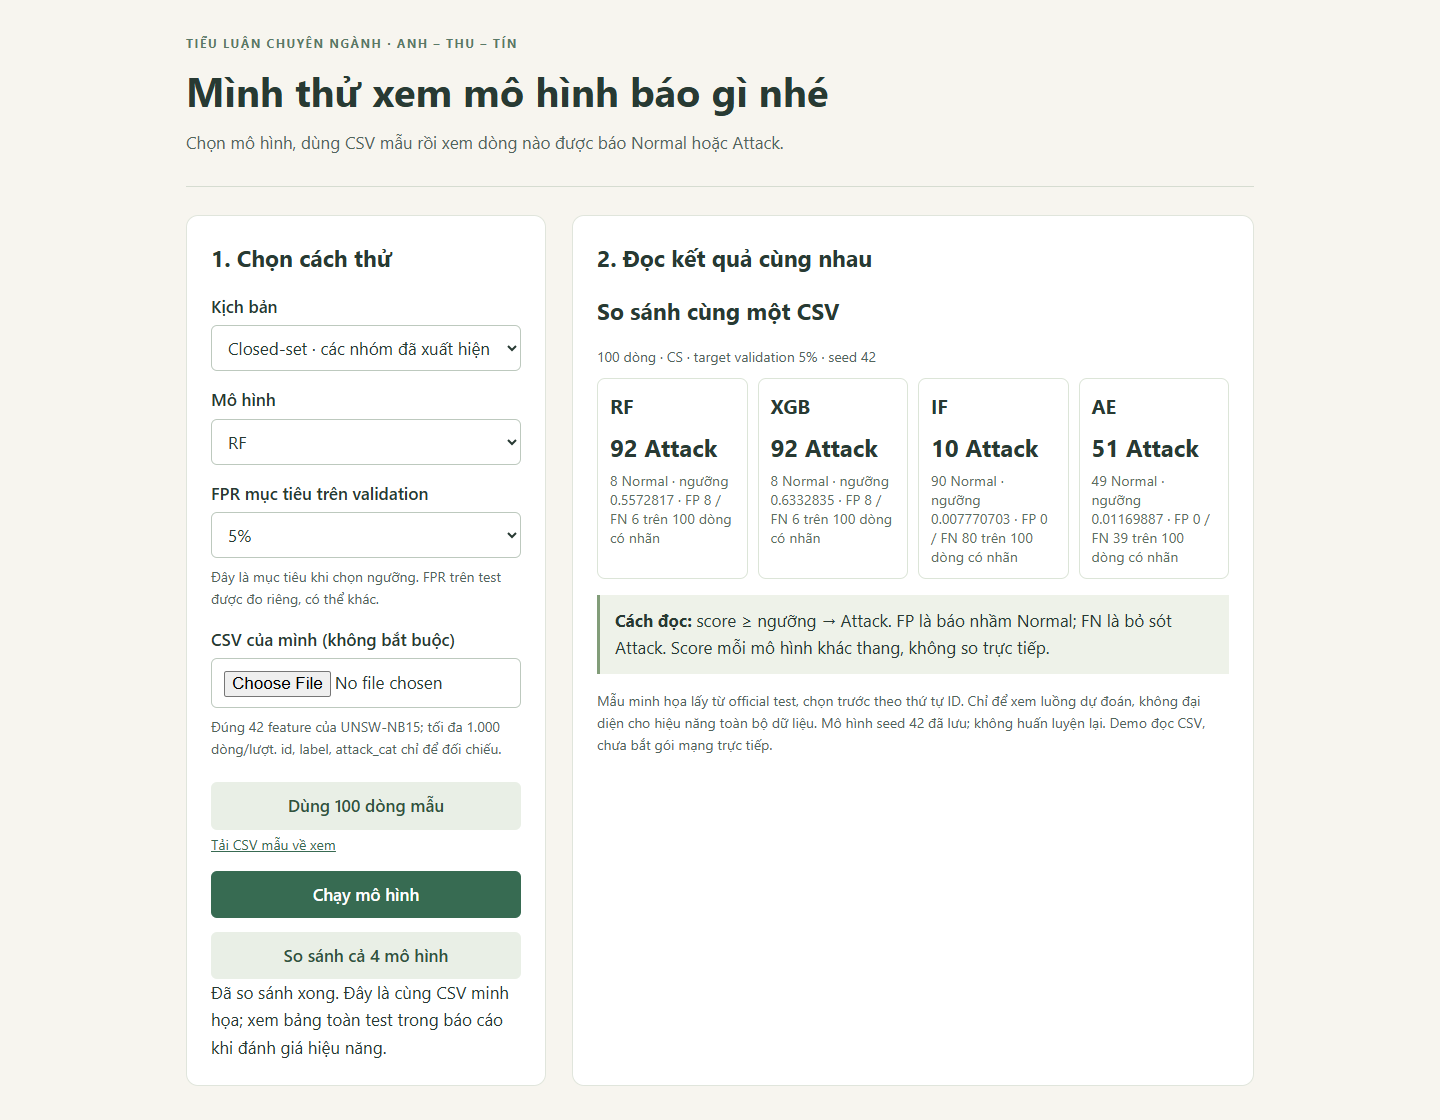
\includegraphics[width=\textwidth]{assets/demo_20261025/DEMO_COMPARISON.png}
\caption[Chức năng so sánh bốn mô hình, ảnh lịch sử ngày 25/10]{Ảnh lịch sử ngày 25/10 của chức năng so sánh bốn mô hình trên cùng CSV mẫu, CS seed 42, target validation 5\%. Đây là giao diện CSV trước bản trình bày ngày 13/11.}
\end{figure}

\section{Kiểm chứng bằng bundle thật}
Lần đối chiếu HTTP ngày 12/11 chạy 16 bundle seed 42 (4 kịch bản $\times$ 4 mô hình), mỗi bundle ở hai ngưỡng: 32 trường hợp $\times$ 100 dòng = 3.200 so sánh dự đoán. Nhãn dự đoán và ngưỡng đều khớp prediction đã khóa. Sai khác score lớn nhất $2.20\times10^{-7}$, dưới dung sai $10^{-6}$; không gọi score là giống từng byte. Bằng chứng tại \path{output/presentation_review_20261112/API_AUDIT.json}. Kiểm lỗi thiếu feature, rỗng, số không hợp lệ và vô cực đều từ chối đầu vào; bundle và prediction gốc không thay đổi.

Log \path{output/presentation_review_20261112/TESTS.log} ghi 46 test đạt. Đây là kiểm hành vi chương trình, không phải 46 thí nghiệm đo chất lượng mô hình. Hồ sơ sửa giao diện ngày 13/11 tại \path{output/presentation_review_20261113/} ghi kiểm dữ liệu có nhãn, không nhãn, một phần nhãn, CSV sai schema, đổi cấu hình và chuyển bản ghi. Nhóm vẫn cần tự thao tác, hiểu nhãn đối chiếu và giải thích giới hạn trước buổi báo cáo.

\section{Ví dụ để tập giải thích}
Với CS--RF--S42, bản ghi 1 có score 0,705741 và nhãn Normal. Ở target validation 5\%, ngưỡng 0,557282 nên mô hình cảnh báo Attack: đây là FP. Chuyển target 1\% rồi chạy lại, ngưỡng tăng lên 0,805367 và cùng score trở thành dự đoán Normal: đây là TN. Mô hình không học lại; ví dụ chỉ thay ngưỡng quyết định.

Bảng sau chọn ID nhỏ nhất của từng nhóm FP/FN từ prediction gốc, không phải cả bốn bản ghi đều thuộc mẫu hỗn hợp 50 dòng. Mỗi ví dụ chỉ minh họa cách đọc nhãn, score và ngưỡng; không suy nguyên nhân lỗi từ importance toàn mô hình.
\begin{table}[H]\centering\small
\caption{Ví dụ score/ngưỡng và lỗi từ prediction thật, target validation 5\%}
\begin{tabular}{L{2.7cm}L{.7cm}L{.7cm}L{3cm}rr}\toprule Run & ID & Lỗi & Nhóm thật & Score & Ngưỡng\\\midrule
CS-RF-S42 & 1 & FP & Normal & 0.705741 & 0.557282\\
CS-IF-S42 & 38 & FP & Normal & 0.018721 & 0.007771\\
CS-IF-S42 & 244 & FN & Reconnaissance & -0.059887 & 0.007771\\
CS-RF-S42 & 278 & FN & Fuzzers & 0.429308 & 0.557282\\
\bottomrule\end{tabular}\end{table}

\section{Khả năng tái lập và phần còn mở}
Repo giữ mã, cấu hình, phiên bản thư viện, bảng run và audit. Raw CSV, mô hình và prediction nặng nằm ở local hoặc kho lưu trữ được chỉ rõ trong hướng dẫn; ZIP nguồn báo cáo không thay gói artifact để chạy mô hình. Các script phân tích đọc kết quả đã lưu, không tự thay 80 run gốc. Bản đợt 3 đã gửi ngày 12/11 được giữ nguyên; bản đợt 4 và tổng cần được đọc duyệt riêng.

Đã có số đo transform+score trên 100 dòng mẫu cho 80 bundle, nhưng chưa đánh giá cảm biến trực tiếp, độ trễ/throughput vận hành, concept drift hay chi phí triển khai. Chưa có thời gian train-only và phần cứng lịch sử; không coi tổng run là train time. Chưa có dataset độc lập, retrain loại overlap hay thẩm định mới từ giảng viên. Hạn nộp theo thông báo chính thức; ngày biên tập không thay ngày thực nghiệm, ngày gửi hoặc bằng chứng đóng góp của thành viên.
